\section{Results}
\label{sec:results}

Table~\ref{tab:main} gathers every \AtoH{} configuration on the held-out set. Where we quote a recovery
$\dlab$ below, it is $W_{\mathrm{LAB}}(\text{raw},\text{target})-W_{\mathrm{LAB}}(\text{output},\text{target})$
on the slide in question, so positive means closer to the real scanner than doing nothing.

\begin{table*}[t]
\centering
\caption{\AtoH{} results on the five held-out slides. LAB Wasserstein (Eq.~\ref{eq:wlab}, lower is
better) and SSIM against the registered Hamamatsu scan; \emph{typical} is A08, A09, A13 and A16. Every
trained method uses the same 50 A03/H03 pairs. Rows marked $^\dagger$ average three seeds (1{,}488
crop-seeds); the rest use one (496 crops). The raw row is computed over the full baseline crop set.
Bold: best normaliser per column.}
\label{tab:main}
\small
\begin{tabular}{llrrrrrr}
\toprule
& & \multicolumn{3}{c}{LAB Wasserstein $\downarrow$} & \multicolumn{3}{c}{SSIM $\uparrow$}\\
\cmidrule(lr){3-5}\cmidrule(lr){6-8}
Group & Method & ALL & typical & A06 & ALL & typical & A06\\
\midrule
Reference & Raw Aperio (no normalisation) & 33.83 & 25.41 & 94.84 & 0.733 & 0.748 & 0.627\\
\midrule
Classical & Macenko~\cite{macenko2009normalisation} & 24.80 & 21.02 & 50.30 & 0.628 & 0.649 & 0.479\\
 & Reinhard~\cite{reinhard2001colortransfer} & 28.02 & 26.79 & 36.34 & 0.681 & 0.701 & 0.545\\
 & Histogram matching & 30.61 & 31.33 & \textbf{25.72} & 0.651 & 0.664 & 0.562\\
\midrule
Learned & StainNet~\cite{kang2021stainnet} & 55.51 & 58.02 & 38.58 & 0.512 & 0.518 & 0.471\\
 & ParamNet~\cite{kang2024paramnet} & 17.27 & \textbf{8.55} & 76.15 & 0.753 & 0.769 & 0.644\\
 & StainGAN~\cite{shaban2019staingan} & \textbf{15.66} & 13.55 & 29.92 & \textbf{0.764} & \textbf{0.772} & \textbf{0.709}\\
\midrule
SD\,1.5 ladder & A0 frozen img2img & 32.89 & 23.65 & 95.22 & 0.285 & 0.299 & 0.186\\
 & A1 + ControlNet (Canny) & 33.10 & 23.88 & 95.35 & 0.389 & 0.408 & 0.260\\
 & A2 + colour LoRA (rank 8) & 32.12 & 22.96 & 93.92 & 0.289 & 0.304 & 0.191\\
 & A3 ControlNet + LoRA & 32.52 & 23.35 & 94.39 & 0.386 & 0.404 & 0.259\\
 & A4 + LCM-LoRA (8 steps) & 33.96 & 24.91 & 95.06 & 0.398 & 0.417 & 0.272\\
 & A5 + histopathology warm-start & 33.96 & 25.29 & 92.46 & 0.389 & 0.407 & 0.265\\
\midrule
This work & Source ControlNet + LoRA, img2img$^\dagger$ & 30.95 & 22.11 & 90.64 & 0.448 & 0.470 & 0.307\\
 & + DDIM inversion$^\dagger$ & 25.10 & 17.98 & 73.12 & 0.496 & 0.514 & 0.373\\
 & + \texttt{ft-mse} decoder$^\dagger$ & 24.53 & 16.86 & 76.32 & 0.557 & 0.574 & 0.438\\
 & + fine-tuned decoder$^\dagger$ & 25.86 & 17.95 & 79.23 & 0.616 & 0.634 & 0.498\\
 & DDIM inversion + F3 fusion & 26.56 & 18.11 & 83.59 & 0.729 & 0.746 & 0.617\\
\bottomrule
\end{tabular}
\end{table*}

\subsection{The ablation ladder}
No rung of the ladder comes close to the classical baselines (Fig.~\ref{fig:ladder}). The colour LoRA (A2) recovers only
$\dlab=+1.72$ pooled, and on typical slides its LAB distance falls from 25.41 to 22.96. ControlNet raises
SSIM by about 0.10 (A0 0.285 to A1 0.389) but does not move colour. LCM-LoRA (A4) and the histopathology
warm-start (A5) cancel the small colour gain. Ranks 4 and 8 differ by only 0.1--0.3 in LAB distance.
Sweeps show why denoising strength is a poor control knob: with 8 LCM steps, strengths 0.50 and 0.60 give
byte-identical outputs, because the number of steps actually run is $\lfloor 8s\rfloor$. Larger strengths
help the outlier A06 (A5 reaches $\dlab=+24.4$ at 0.70) but damage typical slides (A08 $-7.0$), so no
single strength is usable.

\begin{figure}[t]
\centering
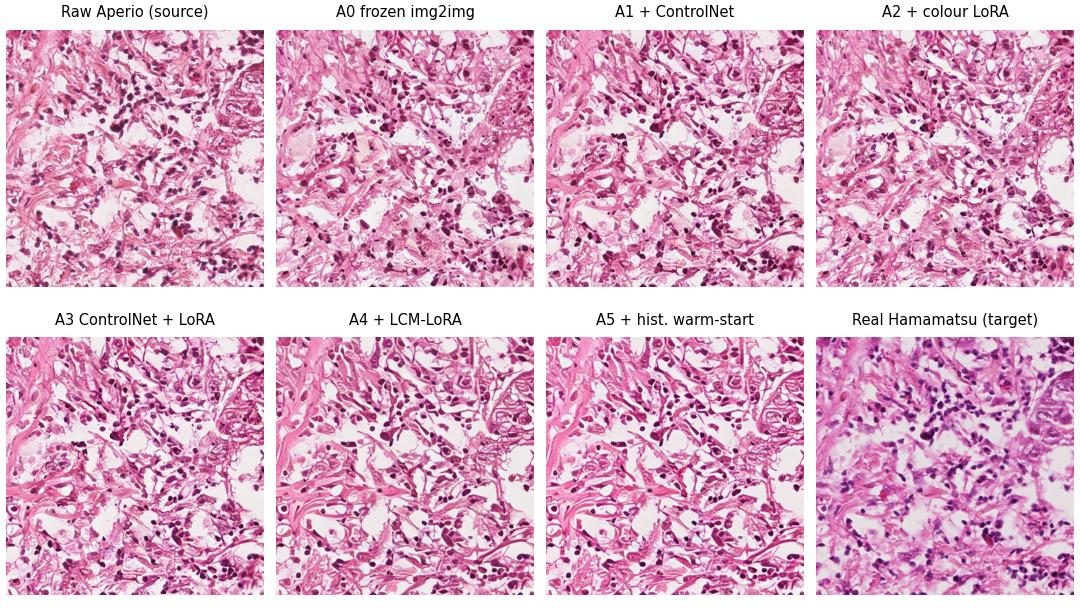
\includegraphics[width=\columnwidth]{ladder_grid_a08.jpg}
\caption{The A0--A5 ladder on a held-out A08 crop (strength 0.30) with the Aperio source and the real
Hamamatsu target. Every rung keeps the source's pink cast; none reaches the target's purple.}
\label{fig:ladder}
\end{figure}

\subsection{Source conditioning and DDIM inversion}
Conditioning on the source image gives a real but modest gain over the ladder ($\dlab=+2.89$, SSIM 0.448).
Replacing random img2img noise with DDIM inversion is the largest single improvement: LAB distance falls to
25.10 pooled and 17.98 on typical slides, every held-out slide moves towards the target (A06 recovery
$+21.7$), and SSIM rises to 0.496. In the reverse direction (\HtoA) the same model fails
($\dlab=-15.6$, a magenta drift), so the gain is direction-dependent.

\subsection{The VAE ceiling}
\label{sec:vae}
SSIM stays far below the raw scan's 0.733 for every diffusion output because the VAE alone cannot
reproduce its input. Self-reconstruction SSIM on the held-out Aperio crops is 0.576 for the stock decoder,
0.618 for \texttt{ft-mse} and 0.646 for our fine-tuned decoder (Fig.~\ref{fig:vaebb}); on Hamamatsu crops it
is 0.726, 0.757 and 0.779, and the fine-tune is highest on every slide (Fig.~\ref{fig:app-vae}). It improves
100\% of Aperio crops, but the limit is generalisation rather than the frozen latent: the same decoder
trained on 16 crops reconstructs those crops at SSIM 0.88. Across backbones the ceiling tracks latent
capacity: SDXL's four-channel VAE reconstructs at only 0.492, while the 16-channel VAE shared by SD\,3.5 and
PixCell reaches 0.773 (eight A06 crops each, so these two are indicative only).

\begin{figure}[t]
\centering
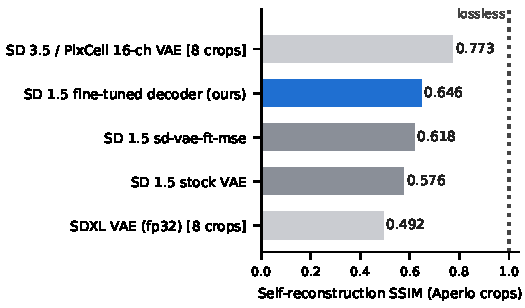
\includegraphics[width=\columnwidth]{vae_backbones.pdf}
\caption{VAE self-reconstruction SSIM, $\mathrm{SSIM}(x, D(E(x)))$, on held-out Aperio crops, across the
backbones used in this work. SD\,1.5 rows use all 496 crops; the SDXL and 16-channel rows use eight A06
crops. Every VAE stays well below the lossless value of 1.0 (dotted).}
\label{fig:vaebb}
\end{figure}

Decoding the DDIM-inversion latents with the better decoders raises translated SSIM from 0.496 to 0.557
(\texttt{ft-mse}) and 0.616 (fine-tuned), winning on every crop-seed. The fine-tune costs colour, though:
typical-slide LAB distance rises from 16.86 to 17.95 and A06 worsens to 79.2. Visual inspection explains
part of the SSIM gain. On two inspected crops the fine-tuned decoder keeps only 21--30\% of the input's
fine-detail energy (Laplacian variance), against 52--59\% for \texttt{ft-mse}, and shifts the blue channel
by 3--5 levels. The real Hamamatsu scans are themselves soft, at 18--24\% of the Aperio source's detail,
so much of the translated SSIM gain comes from matching the target scanner's softness rather than from
recovering structure.

\subsection{Detail fusion}
\textbf{Choosing the variant.} Table~\ref{tab:fusion} compares the three fusion rules and the F3
parameters on internal training-domain crops. These crops are coordinate-corresponding rather than
registered, so absolute SSIM is low and only comparisons within the table are meaningful. Every variant
raises SSIM over the unfused prediction. F1 is worse than F3 on both axes; pasting the prediction's
unblurred chroma onto the source luminance is the likely cause. F2 sits at other points of the trade-off:
more SSIM for much worse colour ($\alpha=0.5$), or the lowest LAB distance at lower SSIM ($\alpha=1$). F3
was chosen as the best balance, and on visual inspection it was indistinguishable from the source in
nuclear boundaries and chromatin, with no haloes, ringing or gamut clipping.

\textbf{What the sweep shows.} SSIM is flat across $\beta$, from $0.10$ to $1.00$, and nearly flat across
$\sigma$ once $\sigma\geq8$. This is the mechanism of Eq.~\eqref{eq:f3} at work: the blurred residual
cannot reach fine structure at any strength, so the structural gain comes from starting at the source
pixels at all. Colour traces a U-shape in $\beta$ with its minimum at 0.5. Small $\beta$ leaves the source
colour almost unchanged, and large $\beta$ adds more of a \emph{smoothed approximation} of the prediction's
shift, which is worse than the shift itself.

\begin{table}[t]
\centering
\caption{Fusion design on internal training-domain crops (SSIM, and LAB Wasserstein against the paired
Hamamatsu crop). Top: the three rules on 50 crops. Bottom: the F3 parameter sweep on 20 crops. Bold: the
frozen configuration.}
\label{tab:fusion}
\footnotesize
\begin{tabular}{llrr}
\toprule
& Configuration & SSIM $\uparrow$ & LAB W. $\downarrow$\\
\midrule
\multicolumn{4}{l}{\emph{Fusion rules, 50 crops}}\\
& Unfused DDIM-inversion prediction & 0.1604 & 22.11\\
& F1, source luminance (Eq.~\ref{eq:f1}) & 0.1826 & 24.63\\
& F2, $\alpha=0.5$ (Eq.~\ref{eq:f2}) & 0.1955 & 30.74\\
& F2, $\alpha=1.0$ & 0.1813 & 20.30\\
& \textbf{F3, $\sigma=8$, $\beta=0.5$} (Eq.~\ref{eq:f3}) & \textbf{0.1854} & \textbf{22.67}\\
\midrule
\multicolumn{4}{l}{\emph{F3 sweep, 20 crops (unfused: 0.1644 / 21.46)}}\\
& $\sigma=8$, $\beta=0.10$ & 0.1866 & 25.63\\
& $\sigma=8$, $\beta=0.25$ & 0.1866 & 23.95\\
& \textbf{$\sigma=8$, $\beta=0.50$} & \textbf{0.1866} & \textbf{21.44}\\
& $\sigma=8$, $\beta=0.75$ & 0.187 & 21.75\\
& $\sigma=8$, $\beta=1.00$ & 0.1865 & 22.50\\
& $\sigma=4$, $\beta=0.75$ & 0.185 & 21.74\\
& $\sigma=16$, $\beta=0.75$ & 0.187 & 21.75\\
\bottomrule
\end{tabular}
\end{table}

\textbf{Held-out result.} Fusing only the learned colour change onto the raw source raises SSIM to 0.729 pooled
and 0.746 on typical slides, above every classical baseline, while keeping most of the colour shift:
typical-slide LAB distance is 18.11 (raw 25.41) and windowed LAB 18.65, closer to the target than Macenko
(21.88), Reinhard (27.42) or histogram matching (31.90). Fig.~\ref{fig:f3} shows the process. A06 benefits
least (LAB 83.6) and stays visibly paler than the Hamamatsu scan. Fusion also absorbs other structural
gains: a three-member self-ensemble raises unfused SSIM from 0.496 to 0.543 but adds nothing after fusion
(0.7288 against 0.7290), and the fine-tuned decoder adds nothing either (0.7289) while worsening fused
windowed LAB from 27.08 to 27.74. In the failed \HtoA{} direction, fusion applied unchanged raises SSIM from
0.548 to 0.730 and shrinks the colour loss from $\dlab=-15.6$ to $-5.3$, although colour is still worse
than doing nothing. It also transfers to SDXL with the same frozen parameters (Table~\ref{tab:sdxl}).

\begin{figure*}[t]
\centering
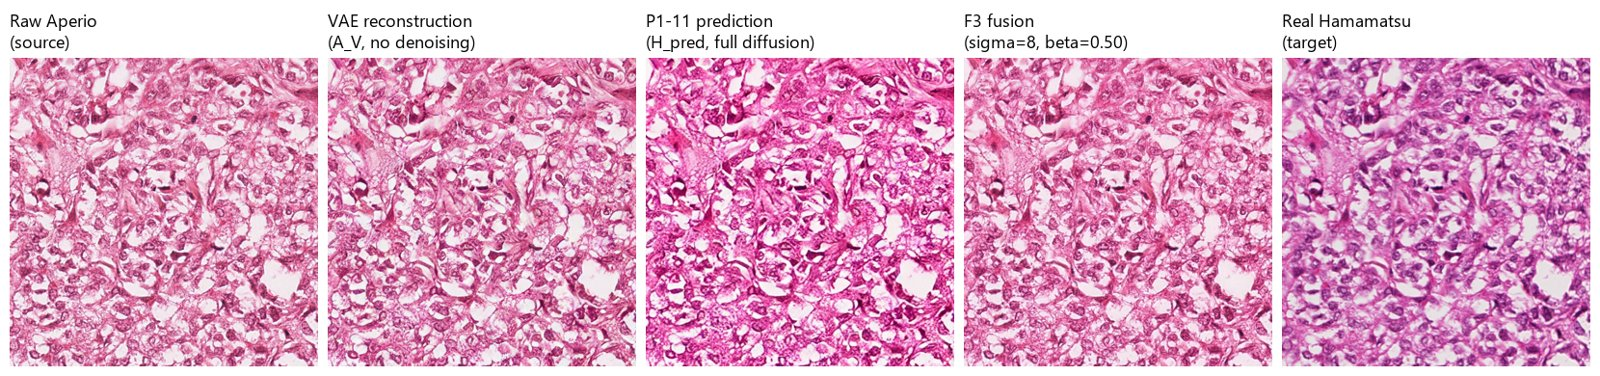
\includegraphics[width=\textwidth]{p1_16_a08.jpg}
\caption{F3 fusion on held-out slide A08: raw Aperio source $A$, its VAE reconstruction $A_V$, the
DDIM-inversion prediction $H_{\mathrm{pred}}$, the fused output (Eq.~\ref{eq:f3}, $\sigma=8$, $\beta=0.5$)
and the registered real Hamamatsu target.}
\label{fig:f3}
\end{figure*}

\subsection{Learned baselines}
Trained on the same 50 pairs, ParamNet and StainGAN outperform every diffusion configuration in
Table~\ref{tab:main} (Fig.~\ref{fig:compare}). ParamNet has the lowest typical-slide LAB distance (8.55) and StainGAN the lowest
pooled distance (15.66) and the highest SSIM (0.764 pooled, 0.709 on A06), above even the raw scan's
pixel similarity. StainNet, a per-pixel 1$\times$1 network with 1{,}283 parameters, is worse than doing
nothing on every typical slide; a 150{,}000-step retrain plateaued at the same training loss, so this is a
capacity limit, not under-training. The ranking holds in the \HtoA{} direction: on typical slides ParamNet
recovers $\dlab=+17.28$ and StainGAN $+10.75$, while StainNet loses $-28.38$. The classical methods only
beat the raw input pooled because of A06: on typical \AtoH{} slides Reinhard ($-1.38$) and histogram
matching ($-5.92$) are slightly worse than doing nothing, and only Macenko gains ($+4.39$). ParamNet is also
the most consistent learned method across the four typical slides ($+9.8$ to $+19.1$ in \AtoH{}).

\begin{figure*}[t]
\centering
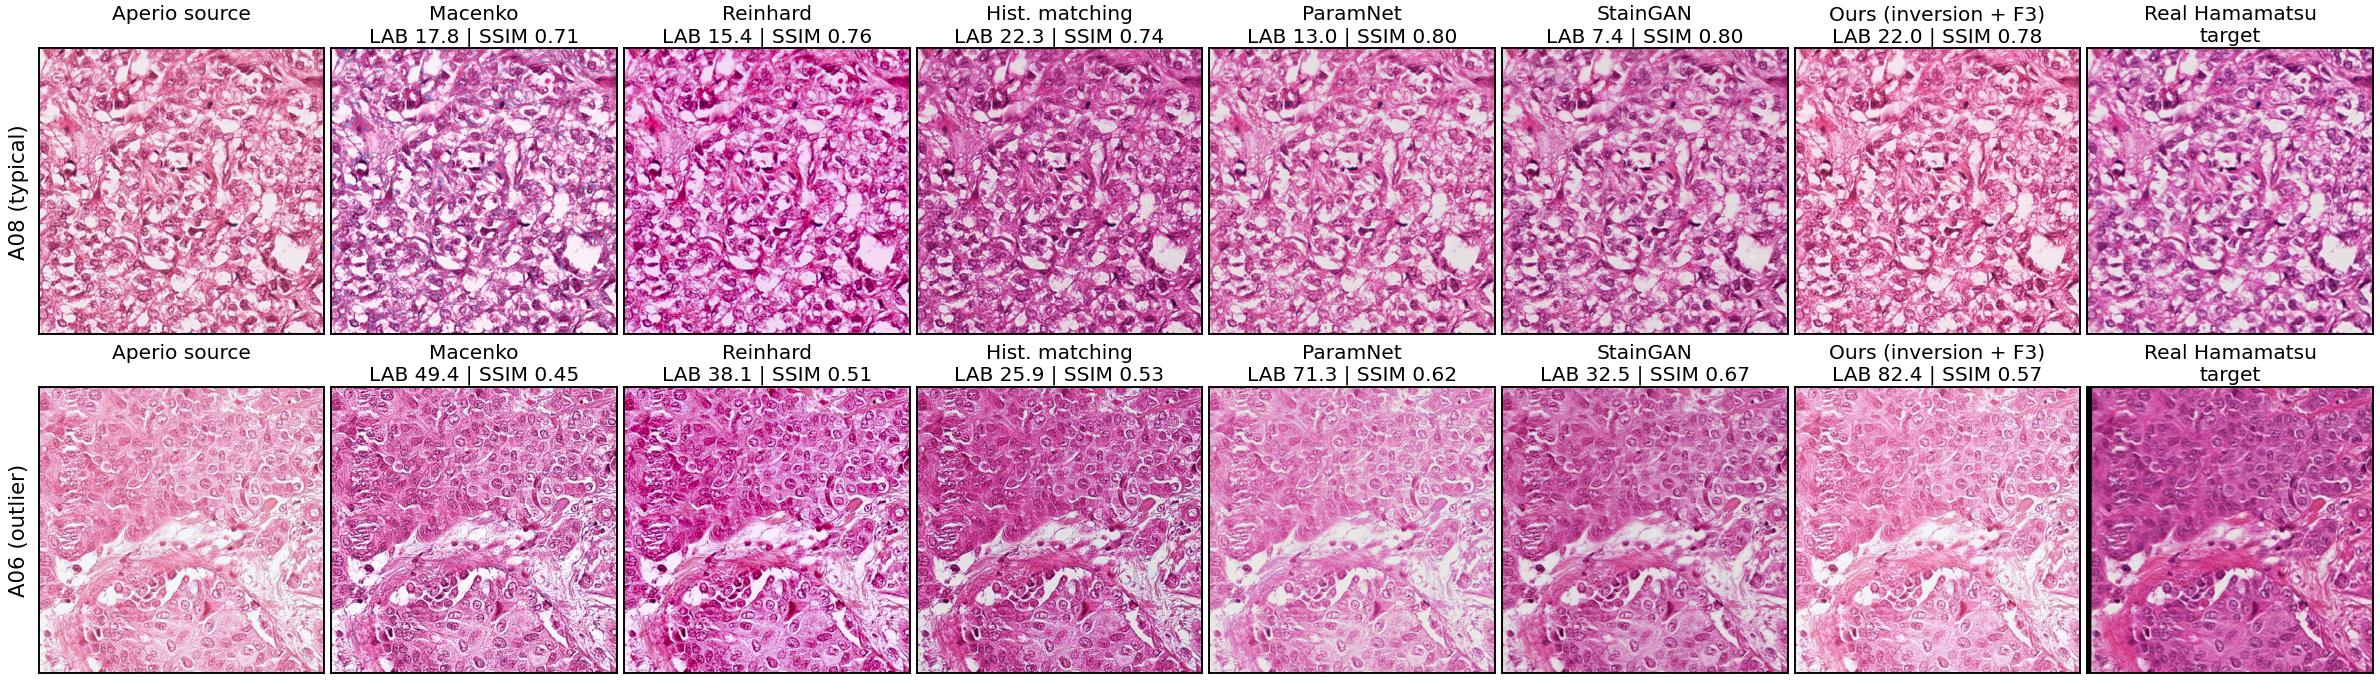
\includegraphics[width=\textwidth]{normaliser_comparison.jpg}
\caption{One held-out crop each from A08 (typical) and A06 (outlier), normalised by every method, with the
per-crop LAB Wasserstein and SSIM against the registered target. These are single crops, not averages:
on this A08 crop our fused output (LAB 22.0) is weaker than its typical-slide mean (18.1). On A06,
ParamNet and our output stay visibly paler than the target, while histogram matching, StainGAN and
Reinhard come closer.}
\label{fig:compare}
\end{figure*}

\begin{table}[t]
\centering
\caption{Structural safety: Relative Dice of HoVer-Net nuclei on 130 Lizard images (95\% bootstrap CI).
Pass threshold 0.95. ``Ours'' is the final pipeline (DDIM inversion + F3 fusion); ``A4-type'' is the
earlier colour LoRA + ControlNet + LCM operating point (strength 0.20).}
\label{tab:reldice}
\small
\begin{tabular}{lrl}
\toprule
Normaliser & Relative Dice & 95\% CI\\
\midrule
ParamNet & \textbf{0.999} & [0.996, 1.001]\\
Ours: inversion + F3 & \textbf{0.994} & [0.992, 0.997]\\
Reinhard & 0.923 & [0.905, 0.939]\\
Diffusion: inversion only & 0.893 & [0.886, 0.900]\\
Diffusion (A4-type) & 0.875 & [0.867, 0.882]\\
Histogram matching & 0.793 & [0.763, 0.822]\\
Macenko & 0.737 & [0.684, 0.787]\\
StainGAN & 0.724 & [0.692, 0.756]\\
StainNet & 0.622 & [0.567, 0.675]\\
\bottomrule
\end{tabular}
\end{table}

\subsection{Structural safety and unseen centres}
Two normalisers pass the Relative Dice gate (Table~\ref{tab:reldice}): ParamNet and our final pipeline
(0.994, 95\% CI $[0.992, 0.997]$, entirely above 0.95). The pass comes from fusion, not from the diffusion
output itself: the unfused inversion output fails at 0.893, and fusion raises Dice on 129 of the 130 images
(mean $+0.071$). This is expected from Eq.~\eqref{eq:f3}, which keeps the source's high frequencies and adds
only a blurred colour change, so nucleus boundaries come from the source. The secondary metrics agree: against
the original images, the fused output keeps IoU (0.535 against 0.539), object-level F1 (0.738 against 0.733) and
the predicted-to-true nucleus count ratio (0.686 against 0.668), while StainGAN lowers object F1 to 0.503 and
the count ratio to 0.384. The earlier A4-type operating point
loses 12.5\% of HoVer-Net's agreement with the ground truth, and StainGAN, despite its high SSIM, loses 28\%,
which is consistent with GANs altering nuclei. On CAMELYON17~\cite{bandi2018camelyon17}, measured as the
mean pairwise LAB distance $D$ between five hospital centres (2{,}103 patches, $D_{\mathrm{pre}}=56.70$), no
SD\,1.5 configuration brings the centres closer. The final pipeline is neutral with fusion
($\Delta D=+0.14$, 95\% bootstrap CI $[-0.22, 0.51]$, 4 of 10 centre pairs improved) and worse without it
($+1.29$ $[0.24, 2.49]$, 3 of 10), as is the A4-type operating point ($+0.83$ $[0.44, 1.19]$, 1 of 10). The CIs
resample the 10 centre pairs, which share centres, so they are supportive only.

\subsection{Downstream clinical utility}
The planned clinical test, an atypia classifier trained on Aperio and scored on normalised Hamamatsu
frames, produced no valid evidence in either direction (Appendix~\ref{app:clinical}). An early result in
which diffusion beat every classical method had been scored in the wrong direction and is retracted. In the
corrected direction no configuration beats the raw input, including our fused pipeline (recovery 0.0, 95\%
CI $[-0.025, +0.025]$). Two rebuilt classifiers, a frozen UNI2-h probe and a criteria-supervised model,
then failed their own pre-registered validity gates, so no atypia number is used as evidence.

\subsection{Few-step inference}
Generic LCM-LoRA on the source-conditioned model is a speed--quality trade-off rather than a match: its best
setting (6 steps, guidance 2.0, strength 0.70) gives A06 SSIM 0.334 and $\dlab=+9.7$, against 0.373 and
$+21.7$ for 50-step DDIM inversion, and A08 0.515/$+3.0$ against 0.537/$+7.2$. Distilling a task-specific
LCM from the source-conditioned teacher was worse than the generic adapter under a pre-committed rule
(paired win rate 30 of 80 crops against 50 of 80).

\subsection{Portability to SDXL}
SDXL transfers the method only with source conditioning and more data than the few-shot budget
(Table~\ref{tab:sdxl}). The ladder configuration (A4) and its warm-started variant (A5) move colour away from
the target, despite SDXL's higher SSIM. Source conditioning works at 512\,px, but natively at 1024\,px the
50-pair model is data-starved: it recovers less colour than doing nothing on every slide, and diagnostics show
that removing its LoRA makes colour worse still, so the adapter helps but is too weak. With 96 or 144 pairs
recovery turns positive, but each extra $\sim$48 pairs adds only about 0.1 in $\dlab$. A source ablation on
the 144-pair model (SSIM 0.318 correct, 0.114 shuffled, 0.109 zero) confirms that it uses the source. F3
fusion transfers unchanged (SSIM 0.732), and with the 144-pair model SDXL passes the CAMELYON17 test with a
small effect ($D_{\mathrm{post}}=54.32$ against $D_{\mathrm{pre}}=56.67$, $\Delta D=-2.35$ $[-2.97, -1.57]$,
9 of 10 centre pairs closer; $-0.67$ $[-0.96, -0.34]$, 8 of 10, with F3 fusion). In
the \HtoA{} direction, where SD\,1.5 fails ($\dlab=-15.6$), SDXL succeeds at both resolutions. Fig.~\ref{fig:sdxl}
shows one crop across the SDXL configurations.

\begin{table}[t]
\centering
\caption{SDXL held-out results (\AtoH{} unless stated; LAB Wasserstein and SSIM as in Table~\ref{tab:main};
source-conditioned rows average three seeds, about 1{,}485 crop-seeds). The 96- and 144-pair runs exceed
the 50-pair budget and are supplementary.}
\label{tab:sdxl}
\footnotesize
\setlength{\tabcolsep}{2.5pt}
\begin{tabular}{lrrrrr}
\toprule
& \multicolumn{3}{c}{LAB W. $\downarrow$} & \multicolumn{2}{c}{SSIM $\uparrow$}\\
\cmidrule(lr){2-4}\cmidrule(lr){5-6}
Configuration & ALL & typ. & A06 & ALL & A06\\
\midrule
Raw Aperio & 33.83 & 25.41 & 94.84 & 0.733 & 0.627\\
A4, strength 0.20 & 39.44 & 30.70 & 98.42 & 0.527 & 0.386\\
A5 warm-start, 0.20 & 39.14 & 30.36 & 98.40 & 0.526 & 0.385\\
Source-cond., 512\,px, 50 pairs & 32.62 & 23.81 & 92.14 & 0.392 & 0.257\\
Source-cond., 1024\,px, 50 pairs & 39.43 & 30.85 & 98.32 & 0.431 & 0.313\\
\quad 96 pairs & 32.51 & 23.79 & 92.29 & 0.442 & 0.322\\
\quad 144 overlapping pairs & 32.40 & 23.80 & 91.42 & 0.446 & 0.335\\
\quad 144 pairs + F3 fusion & 31.78 & 23.06 & 91.62 & 0.732 & 0.638\\
\midrule
\HtoA{}, 512\,px & 24.90 & 17.33 & 75.99 & 0.355 & 0.239\\
\HtoA{}, 1024\,px & 25.17 & 16.68 & 82.47 & 0.386 & 0.274\\
\bottomrule
\end{tabular}
\end{table}

\begin{figure*}[t]
\centering
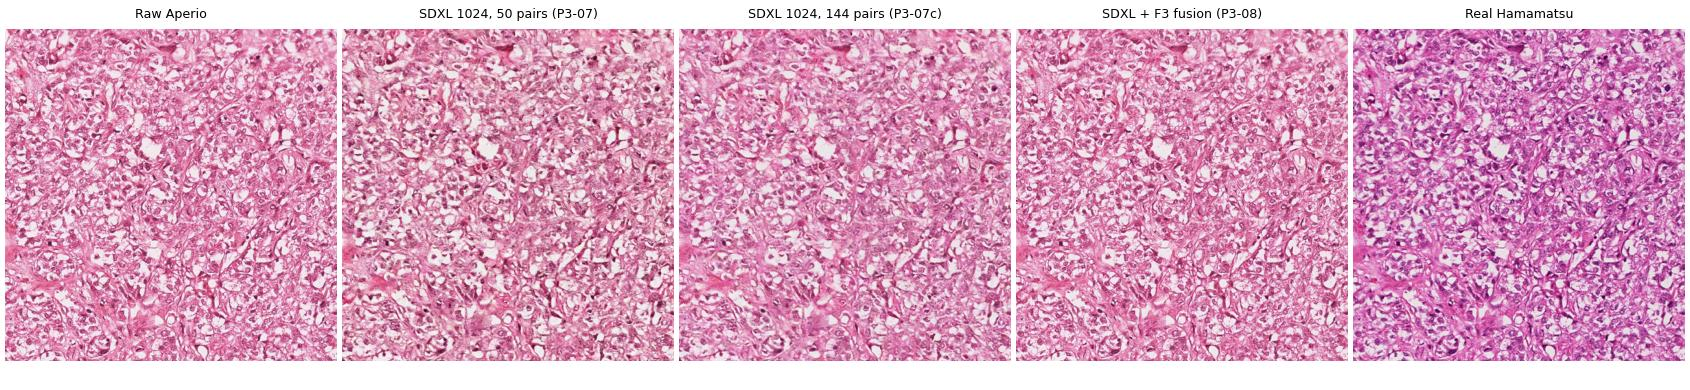
\includegraphics[width=\textwidth]{sdxl_panel_a08.jpg}
\caption{SDXL at native 1024\,px on one held-out A08 crop (frame 00A, origin (0,0), seed 0): raw Aperio,
the 50-pair and 144-pair source-conditioned models, the 144-pair model with F3 fusion, and the registered real
Hamamatsu target. All SDXL outputs stay close to the Aperio colour.}
\label{fig:sdxl}
\end{figure*}

\subsection{Newer backbones (exploratory probes)}
Both newer backbones are feasible to adapt but not yet useful (Table~\ref{tab:cost}). An SD\,3.5-large
rank-8 LoRA trains in about five times SD\,1.5's time and fits a 24\,GB GPU. On 20 A06 crops at 1024\,px
(strength 0.30, without the T5 text encoder to save memory) it recovers $\dlab=+4.77$ but reaches only SSIM
0.183, far below SD\,1.5 and SDXL; because this covers only the outlier slide it is not a general result.
PixCell is the cheapest backbone to adapt and its 16-channel VAE has the highest reconstruction ceiling
(0.773, Fig.~\ref{fig:vaebb}). But generation from a crop's own UNI2-h embedding, without fine-tuning,
scores SSIM 0.045 against the registered target and 0.036 against its own source: a single global embedding
carries no information about where nuclei are (Fig.~\ref{fig:app-pixcell}). Using it for normalisation would
need a source-image conditioning branch for a diffusion transformer, which was not built.

\begin{table}[t]
\centering
\caption{Cost of a rank-8 LoRA, 1{,}000 steps, on one RTX~3090 (exploratory probes).}
\label{tab:cost}
\footnotesize
\begin{tabular}{lrrr}
\toprule
& SD\,1.5 & SD\,3.5-large & PixCell\\
\midrule
Wall-clock (s) & 160.5 & 798.8 & \textbf{130.3}\\
Peak VRAM (GB) & -- & 17.77 & \textbf{4.20}\\
Trainable parameters & 1.59M & 5.91M & 2.06M\\
\bottomrule
\end{tabular}
\end{table}
